\section{Przypadek Testowy 1 - Algorytm genetyczny - zależność PRD od liczby iteracji}
  \subsection{Cel:}
    W tej części zostaną ze sobą porównane PRD rozwiązania algorytmu genetycznego w zależności od liczby iteracji.
    \subsection{Założenia:}
    Do badania tego przypadku została wykorzystana instancje 
    \begin{itemize}
      \item berlin52.tsp
      \item eil76.tsp
      \item eil51.tsp
      \item gr17.tsp
      \item gr21.tsp
      \item gr24.tsp
      \item gr48.tsp
      \item hk48.tsp
      \item kroA100.tsp
      \item kroA150.tsp
      \item kroB100.tsp
      \item kroB150.tsp
      \item swiss42.tsp
      \item ftv33.atsp
      \item ftv35.atsp
      \item ftv38.atsp
      \item ftv44.atsp
      \item ftv47.atsp
      \item br17.atsp
    \end{itemize}
    Dodatkowo współczynnik mutacji został ustalony na 0.2, współczynnik selekcji na 0.7. Ponad to wielkość populacji została ustalona na 100. Badane iteracje były z zakresu {100, 200, 300, ... 1000}.
  \subsection{Wyniki: }
  Poniższa tabela przedstawia wyniki testów - średnie PRD (w procentach), odchylenie standardowe oraz błęd standardowy. 
  
  \begin{table}[!ht]
    \centering
    \begin{tabular}{|l|l|l|l|}
    \hline
        Iterations & PRD & SD & SE \\ \hline
        100 & 136.24 & 143.32 & 33.78 \\ \hline
        200 & 93.97 & 106.53 & 25.11 \\ \hline
        300 & 68.04 & 78.38 & 18.48 \\ \hline
        400 & 55.14 & 66.65 & 15.71 \\ \hline
        500 & 47.74 & 56.61 & 13.34 \\ \hline
        600 & 40.10 & 44.34 & 10.45 \\ \hline
        700 & 35.53 & 37.29 & 8.79 \\ \hline
        800 & 30.60 & 31.65 & 7.46 \\ \hline
        900 & 29.82 & 29.68 & 7.00 \\ \hline
        1000 & 31.33 & 32.55 & 7.67 \\ \hline
    \end{tabular}
    \caption{PRD - uśrednione wyniki, SD - odchylenie standardowe, SE - Błąd standardowy}
  \end{table}

  Odchylenie standardowe oraz błąd standardowy zostały obliczone według wzorów: \\
    Odchylenie standardowe:
    \[ \sigma = \sqrt{\frac{\sum_{n = 1}^{18}(\bar{x} - x_n)^2}{18}} \]
    Błąd standardowe:
    \[ \sigma_{\bar{x}} = \frac{\sigma}{\sqrt{18}} \]

  \subsection{Wykresy: }
    \begin{figure}[H]
      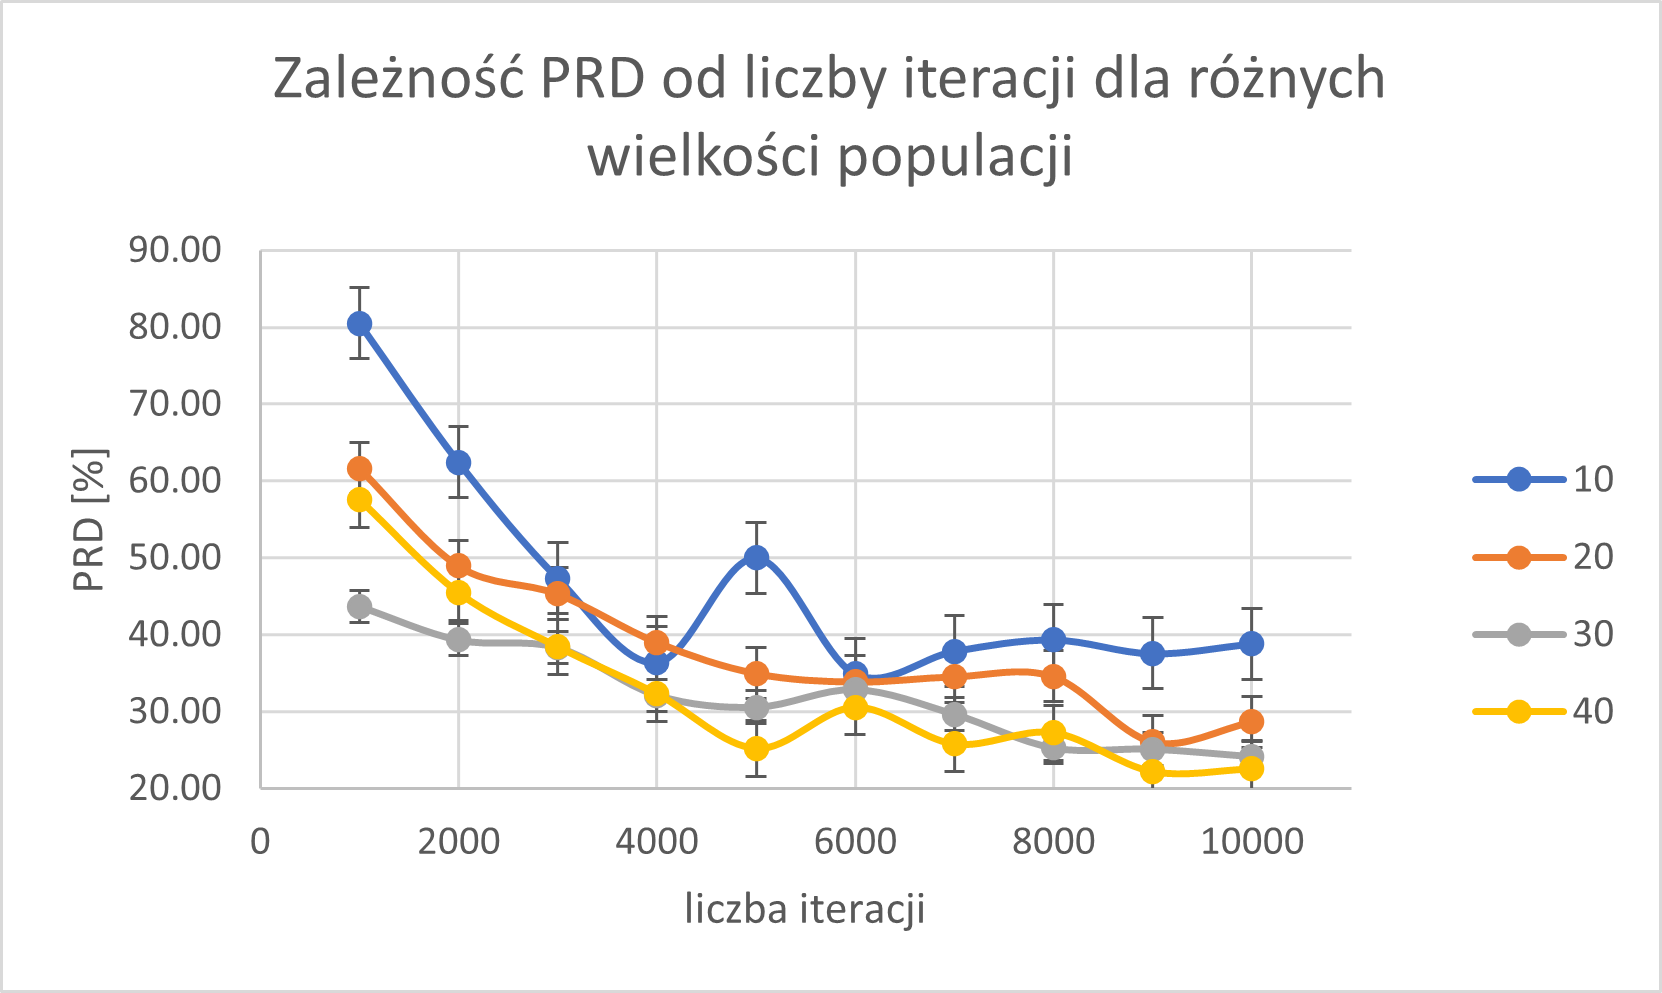
\includegraphics[scale=0.75]{chart_test_1.png}
      \centering
      \caption{Zależność PRD od liczby iteracji dla różnych wielkości populacji}
    \end{figure}
  
  Na wykresie przedstawione są średnie wartości PRD dla badanych danych. Uśrednione wartości PRD maleją logarytmicznie, wraz ze wzrostem liczby iteracji.

  \subsection{Wnioski: }
  Zgodnie z oczyekiwaniami, zwiękaszanie liczby iteracji zwiększa jakość rozwiązań. wartości maleją logarytmicznie od liczby iteracji, zgodnie z zaznaczoną linią trendu. Ponadto wraz ze wzrostem liczby iteracji zmiejsza się odchylenie standardowe oraz błąd standardowy wyników.

